\section{Manuel utilisateur}
\label{sec:manuel}

Bienvenue dans le manuel utilisateur de Glasir, un logiciel d'aide aux experts en sécurité basé sur le formalisme des ADTrees\footnote{Abréviation d'\og Attack-Defense Trees \fg{}, ou \og Arbres d'Attaque et de Défense\fg{} en français.}. Grâce à Glasir, vous pourrez analyser efficacement vos ADTrees préalablement créés avec ADTool~\cite{adtool}, un logiciel open-source disponible sur Internet.

Ce manuel commencera par décrire le fonctionnement général du logiciel (création d'un nouveau projet, ouverture d'un projet existant, etc.), avant d'expliquer comment prendre en main les trois fonctionnalités principales que sont l'Éditeur de fonctions, le Filtre et l'Optimiseur. 

Après cela, dans la {\sc sous-section}~\ref{ssec:manuelADTool} vous trouverez des détails concernant l'utilisation d'ADTool, surtout les nouveautés qui lui ont été ajoutées lors de ce projet.

	\begin{figure}[!h]
        \centering
        
\includegraphics[height=0.3\textwidth]{figure/glasir.png}
    \end{figure}

\subsection{Glasir}
\label{ssec:manuelGlasir}

\paragraph{Agencement général de la fenêtre}
Lorsque vous démarrez Glasir, la fenêtre présentée sur la {\sc Figure}~\ref{fig:princ} s'affiche. Nous allons décrire rapidement la structure de cette fenêtre, sans rentrer dans les détails : 
\begin{itemize}
	\item  la barre de menu située en haut vous permet d'ouvrir des ADTrees, de sauvegarder des projets, ou encore d'obtenir des indications si vous avez besoin d'aide;
	\item le bloc central vous permet d'accéder à l'Éditeur de fonction (\emph{FunctionEditor}), au Filtre (\emph{Filter}) et à l'Optimiseur (\emph{Optimize});
	\item la ligne de texte en dessous du bloc central indique sur quel ADTree vous travaillez. Au démarrage, comme aucun ADTree n'est ouvert, le message \og No ADTree selected \fg{} est initialement affiché.
	\item le bloc en bas, surmonté du message \og ADTrees available \fg{}, vous indique quels sont les ADTrees appartenant au porjet courant. Comme aucun projet n'est ouvert au démarrage, ce bloc est initialement vide.
	\item la case cochable \emph{Show complete path}, tout en bas, vous permet d'afficher le chemin complet des ADTrees listé dans le bloc situé au-dessus.
	\end{itemize}
	
	Nous allons maintenant détailler le fonctionnement de chacune des fonctionnalités de Glasir.
	
	\begin{figure}[!h]
        \centering
        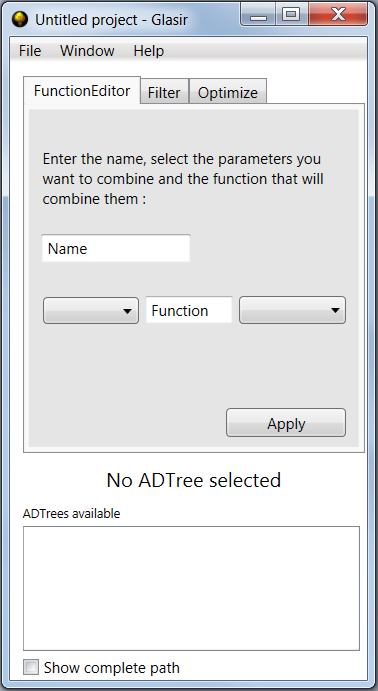
\includegraphics[height=0.7\textwidth]{figure/glasirFenetrePrincipale.png}
        \caption{Fenêtre principale s'affichant au démarrage de Glasir.}
        \label{fig:princ}
    \end{figure}

\paragraph{Ouvrir un ADTree}
Pour ouvrir un ADTree, cliquez sur le bouton \emph{File} situé tout en haut à gauche, dans la barre de menu. Puis, dans le menu déroulant, cliquez sur \emph{Open ADTree File}, comme indiqué sur la {\sc Figure}~\ref{fig:file}. Une boîte de dialogue apparaît : parcourez vos dossiers pour sélectionner l'ADTree que vous souhaitez ouvrir. Notez que seul les ADTrees au format XML sont supportés par Glasir. Une fois l'ADTree sélectionné, cliquez sur le bouton \emph{Open} de la boite de dialogue. ADTool se lance alors pour afficher votre ADTree. Notez qu'au démarrage, cette opération peut prendre quelques secondes. Une fois ADTool lancé, Glasir se présente sous la forme de plusieurs fenêtres, comme indiqué sur la {\sc Figure}~\ref{fig:gladitoule}. Si la fenêtre d'ADTool ne s'affiche pas au bout d'une minute ou qu'un autre programme qu'ADTool se lance, c'est que vos fichier \emph{.jar} ne sont pas associés à Java (ou que vous ne possédez simplement pas Java). Consultez et suivez les étapes du fichier \emph{ReadMe.txt} (en anglais) fourni avec Glasir pour obtenir des informations supplémentaires et corriger le problème.

	\begin{figure}[!h]
        \centering
        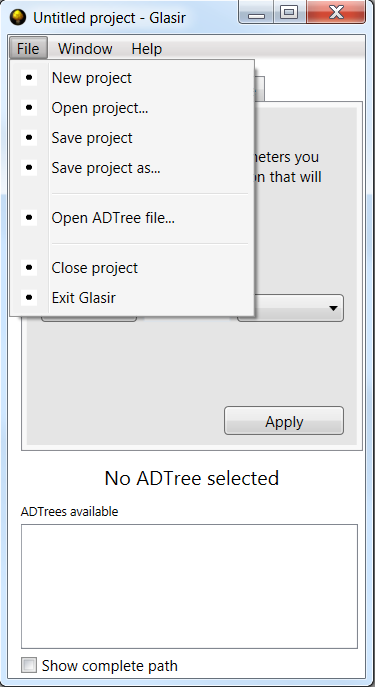
\includegraphics[height=0.7\textwidth]{figure/openfile.png}
        \caption{Menu déroulant disponible en cliquant sur le bouton \emph{File} de la barre de menu.}
        \label{fig:file}
    \end{figure}
    
    \begin{figure}[!h]
        \centering
        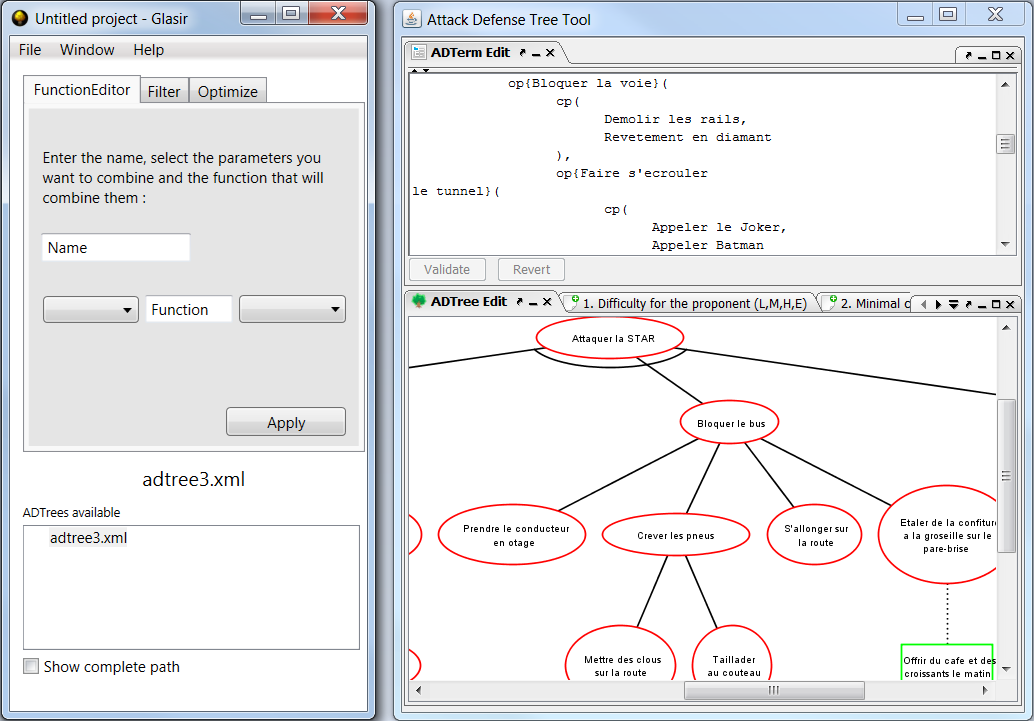
\includegraphics[height=0.7\textwidth]{figure/glasirAditoule.png}
        \caption{Fenêtres visibles après ouverture d'un ADTree.}
        \label{fig:gladitoule}
    \end{figure}

\paragraph{Enregistrer un projet} Lorsque vous avez ouvert un ou plusieurs ADTrees, vous avez la possibilité de sauvegarder l'état actuel de votre projet, c'est-à-dire la liste des ADTrees ouverts. Pour ce faire, cliquez sur \emph{File}, puis sur \emph{Save project as} pour choisir l'emplacement où enregistrer le fichier du projet. Donnez-lui un nom, puis cliquez sur le bouton \emph{Save} de la boite de dialogue. Une fois ceci fait, le titre de la fenêtre de Glasir portera alors le nom de votre projet. Vous pourrez par la suite cliquer directement sur \emph{Save project} pour enregistrer vos modifications.

\paragraph{Ouvrir un projet} Si vous avez déjà un projet enregistré, c'est-à-dire un fichier avec l'extension \emph{.glpf} (\emph{Glasir Project File}), vous pouvez recharger ce fichier : cliquez sur \emph{File}, puis \emph{Open project}. Parcourez vos dossiers pour retrouver votre fichier de projet, sélectionnez-le, puis cliquez sur le bouton \emph{Open} de la boite de dialogue. Si vous aviez un projet ou des ADTrees ouverts, ils seront fermés pour que votre projet enregistré puisse être ré-ouvert. Notez que toute modification non-sauvegardée ne sera pas enregistrée lors de la fermeture.

\paragraph{Aide} Si vous avez des problèmes avec le lancement d'ADTool, vous pouvez cliquer sur le bouton \emph{Help} de la barre de menu pour obtenir des informations supplémentaires. Nous vous invitons dans ce cas à suivre les consignes indiquées dans le fichier \emph{ReadMe.txt} (en anglais) fourni avec Glasir.

\paragraph{Changer d'ADTree courant} Pour pouvoir utiliser les modules de Glasir, vous devez sélectionner un ADTree courant, sur lequel les opérations des modules seront appliquées. Le bloc en bas de la fenêtre principale dresse la liste des ADTrees de votre projet.  Vous avez la possibilité de cocher la case \emph{Show complete path}, en bas, pour voir le chemin complet de chaque ADTree. Cliquez sur un ADTree dans la liste pour qu'il devienne l'ADTree courant. Son nom est alors indiqué à la ligne du dessus, en plus gros. Si aucun ADTree n'est disponible ou sélectionné, le message \og No ADTree selected \fg{} est affiché à la place. Notez que lorsque vous ouvrez un ADTree, ce dernier devient automatiquement l'ADTree courant.

\paragraph{Éditeur de fonctions}Cette fonctionnalité a pour intérêt d'exprimer un compromis entre deux valuations d'un ADTree en en créant une troisième, fonction des deux premières. Par exemple, si vous avez un ADTree qui a comme paramètres \og Minimal cost for the proponent \fg (en euros) et \og Minimal time for the proponent (sequentiall) \fg (en heures) et que vous estimez que une heure \og coute \fg par comparaison 20 euros, vous pouvez créer un nouveau paramètre de type \og Minimal cost for the proponent \fg exprimant un compromis entre les deux paramètres qui sera égal à coût+20*temps.

 \begin{figure}[!h]
        \centering
        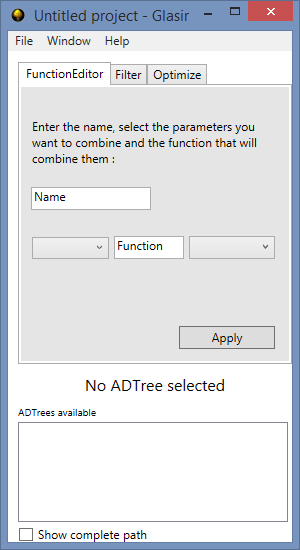
\includegraphics[height=0.7\textwidth]{figure/functionEdition.png}
        \caption{Onglet FunctionEditor.}
        \label{fig:functEdit}
    \end{figure}

Pour utiliser l'éditeur de onctions, suivez les étapes suivantes : 
\begin{itemize}
\item Assurer vous d'avoir l'ADTree que vous voulez utiliser d'ouvert et désigné comme l'arbre courant. 
\item Sélectionnez l'onglet \og FunctionEditor \fg .
\item Sélectionnez les deux paramètres de l'ADTree que vous voulez combiner au moyen des deux ComboBox présentent dans l'onglet. ATTENTION  ! : le nouveau paramètre aura pour type celui du premier paramètre sélectionné (à gauche), par exemple si le premier paramètre est de type \og Minimal time for the proponent (sequentiall) \fg , alors le nouveau paramètre calculé le sera aussi. Si vous sélectionnez un paramètre de type discret, un nombre de cases égal au nombre valeurs possibles s'affichera. Vous pourrez alors pondérer ces valeurs de la plus petite (à gauche), à la plus grande (à droite).
\item Inscrivez dans la textBox \og Function \fg la fonction que vous voulez utiliser pour le calcul du nouveau paramètre. Par exemple, si vous voulez faire \og newParam = firstParam + 2*secondParam\fg , inscrivez \og +2*\fg .
\item Entrez le nom que vous voulez donné au nouveau paramètre créé dans la textBox \og Name\fg.
\item Enfin, cliquez sur le bouton \og Apply\fg pour créer le nouveau paramètre.
\end{itemize} 
S'ouvrira alors un nouvel arbre dans une nouvelle fenêtre d'ADTool qui sera nommé comme l'arbre utilisé suivi de \og .functEdit\fg . Le nouvel arbre sera enregistré dans le répertoire où se trouve le logiciel Glasir. 
Si un problème survient, l'exécution sera interrompu et une boite de message apparaitra pour vous expliquer pourquoi.

\paragraph{Filtre}Cette fonctionnalité sert a élaguer les chemins d'un ADTree qui ne respectent pas une certaine condition. Par exemple si un ADTree a comme paramètre \og Minimal cost for the proponent \fg (en euros) et que l'on sait qu'un attaquant potentiel ne peut pas dépenser plus de 2000 euros, le filtre permettra alors d'élaguer l'ADTree de manière a ne conserver que les feuilles de l'arbre qui apparaissent dans au moins un chemin permettant d'accomplir l'attaque avec 2000 euros ou moins.

 \begin{figure}[!h]
        \centering
        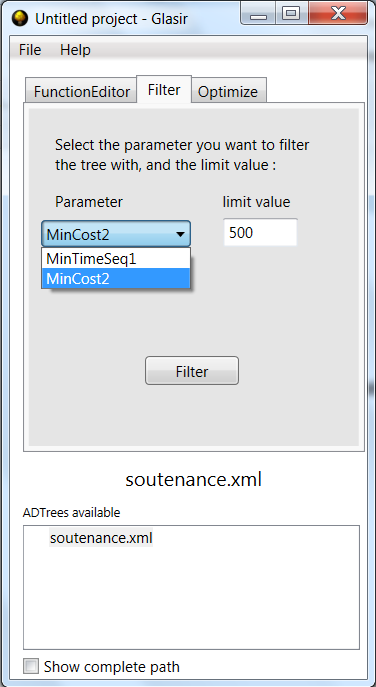
\includegraphics[height=0.7\textwidth]{figure/filter.png}
        \caption{Onglet Filter.}
        \label{fig:filter}
    \end{figure}

Pour utiliser le filtre, suivez les étapes suivantes :

\begin{itemize}
\item Assurer vous d'avoir l'ADTree que vous voulez filtrer d'ouvert et désigné comme l'arbre courant. 
\item Sélectionnez l'onglet \og Filter \fg .
\item Sélectionnez le paramètre selon lequel vous voulez filtre l'arbre avec la ComboBox présente dans l'onglet.
\item Indiquer dans la textBox \og Limit Value\fg la pire valeur acceptable par le filtre pour le paramètre sélectionné. Vous pouvez rentrez une valeur textuelle correspondant à l'une des valeurs de l'ensemble du paramètre si l'ensemble est discret.
\item Enfin, cliquez sur le bouton \og Filter\fg pour filtrer l'arbre.
\end{itemize}
S'ouvrira alors un nouvel arbre correspondant à l'arbre élagué dans une nouvelle fenêtre d'ADTool, qui sera nommé comme l'arbre utilisé suivi de \og .filter\fg . Le nouvel arbre sera enregistré dans le répertoire où se trouve le logiciel Glasir.
Si un problème survient, l'exécution sera interrompu et une boite de message apparaitra pour vous expliquer pourquoi.

\paragraph{Optimiseur}Cette fonctionnalité sert a élaguer les chemins d'un ADTree de manière a ne conserver que le ou les meilleurs chemins selon un paramètre donné. Par exemple si un ADTree a comme paramètre \og Minimal cost for the proponent \fg (en euros) et que l'attaque la moins chère coute 2000 euros, l'optimiseur permettra alors d'élaguer l'ADTree de manière a ne conserver que les feuilles de l'arbre qui apparaissent dans au moins un chemin permettant d'accomplir l'attaque avec 2000 euros seulement.

 \begin{figure}[!h]
        \centering
        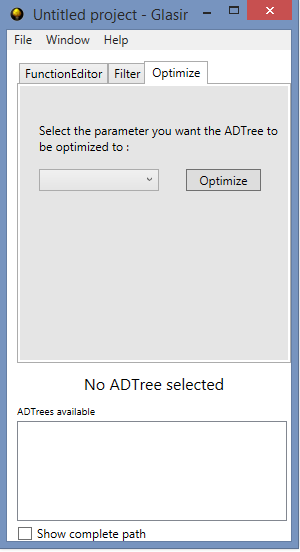
\includegraphics[height=0.7\textwidth]{figure/optimizer.png}
        \caption{Onglet Optimize.}
        \label{fig:opti}
    \end{figure}

Pour utiliser l'optimiseur, suivez les étapes suivantes :
\begin{itemize}
\item Assurer vous d'avoir l'ADTree que vous voulez filtrer d'ouvert et désigné comme l'arbre courant. 
\item Sélectionnez l'onglet \og Optimize \fg .
\item Sélectionnez le paramètre selon lequel vous voulez optimiser l'arbre avec la ComboBox présente dans l'onglet.
\item Enfin, cliquez sur le bouton \og Optimize\fg pour filtrer l'arbre.
\end{itemize}
S'ouvrira alors un nouvel arbre correspondant à l'arbre élagué dans une nouvelle fenêtre d'ADTool, qui sera nommé comme l'arbre utilisé suivi de \og .Optimizer\fg . Le nouvel arbre sera enregistré dans le répertoire où se trouve le logiciel Glasir.
Si un problème survient, l'exécution sera interrompu et une boite de message apparaitra pour vous expliquer pourquoi.

\subsection{Nouvelles fonctionnalités d'ADTool}
\label{ssec:manuelADTool}

Pour le fonctionnement basique d'ADTool, vous pouvez vous référer au manuel utilisateur officiel disponible sur Internet\footnote{Voir à l'adresse suivante : http://satoss.uni.lu/members/piotr/adtool/manual.pdf}. Le guide ici présent ne détaillera que l'utilisation des nouvelles fonctionnalités d'ADTool, qui sont le copier/couper/coller ainsi que l'annulation d'une action.

\paragraph{Copier/couper/coller} Ces fonctionnalités vous seront utiles si vous désirez couper/copier un sous-arbre de l'ADTree courant afin de le coller ensuite à un autre emplacement dans ce même ADTree. Il est à noter que le sous-arbre coupé/copié sera ajouté en tant que fils du n\oe{}ud auquel il sera collé. Aussi, la racine du sous-arbre coupé/copié doit être du même type (opponent ou proponent) que son futur n\oe{}ud parent. Pour couper/copier un sous-arbre puis le coller, suivez les étapes suivantes : 
\begin{enumerate}
    \item Sélectionnez à l'aide d'un clic gauche le n\oe{}ud racine du sous-arbre que vous désirez couper/copier. Si vous avez déjà sélectionné un n\oe{}ud dans l'arbre, vous pouvez également vous déplacer jusqu'au n\oe{}ud souhaité à l'aide des flèches (haut, bas, gauche, droite) du clavier.
	\item Effectuez un clic droit sur le n\oe{}ud sélectionné. Un menu déroulant doit apparaître à côté du n\oe{}ud sélectionné, comme sur la {\sc Figure}~\ref{fig:clicdroit}.
	\item Sélectionnez l'option \og Copy Subtree \fg{}/\og Cut Subtree \fg{}) dans le menu déroulant. Vous pouvez également effectuer cette étape à l'aide d'un raccourci clavier, {\sc CTRL+C}/{\sc CTRL+X}.
	\item Effectuez un clic droit sur le n\oe{}ud auquel vous voulez coller le sous-arbre coupé/copié, puis sélectionnez dans la liste déroulante \og Paste Subtree as Child \fg{}. Si cette option n'apparaît pas dans le menu déroulant, c'est que vous n'avez pas préalablement coupé/copié de sous-arbre. Vous pouvez ici encore utiliser un raccourci clavier, {\sc CTRL+V}.
\end{enumerate}

    \begin{figure}[!h]
        \centering
        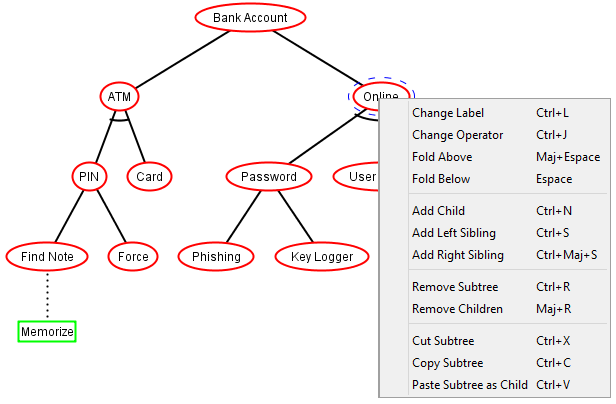
\includegraphics[height=0.7\textwidth]{figure/clicdroit.png}
        \caption{Menu déroulant apparaissant après un clic droit sur un n\oe{}ud.}
        \label{fig:clicdroit}
    \end{figure}

\paragraph{Annulation d'une action} Il s'agit ici d'annuler une ou plusieurs action(s) effectuée(s) précédemment sur l'ADTree courant. Pour cela, il vous suffit tout simplement d'utiliser le raccourci clavier {\sc CTRL+Z} autant de fois que nécessaire, jusqu'à retrouver l'état souhaité pour l'ADTree. Vous pouvez également cliquer sur l'icône \og Undo last action (CTRL+Z) \fg{} en haut à gauche de la fenêtre principale d'ADTool, encadrée en rouge sur la {\sc figure}~\ref{fig:undo}. Les actions pouvant être annulées sont les changements de labels, les ajouts ou suppressions de n\oe{}uds, les changements d'opérateur (conjonction ou disjonction) ainsi que les actions de couper/copier/coller.

\begin{figure}[!h]
        \centering
        
\includegraphics[height=0.17\textwidth]{figure/undo.png}
        \caption{Icône permettant d'annuler l'action précédente.}
        \label{fig:undo}
    \end{figure}